\section{Simulation Results}

\subsection{Block Diagram of the System}

\begin{figure}[H]
    \centering
    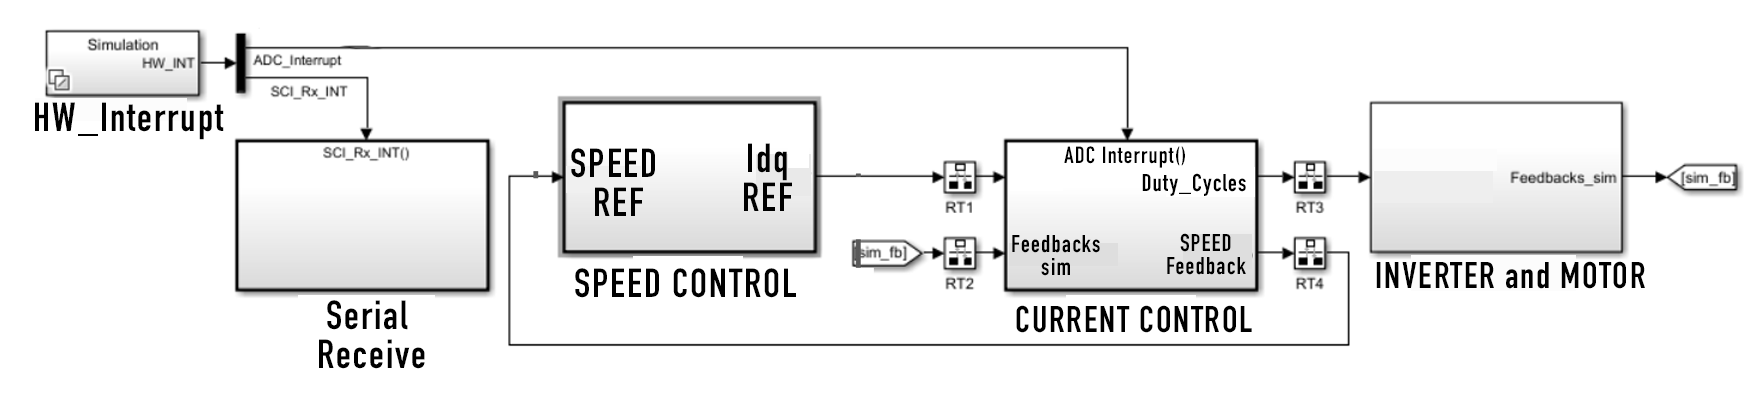
\includegraphics[width=6in]{sections/section3/images/simulation/blockDia.png}
    \caption{Block Diagram of the System}
    \label{fig:block_diagram}
\end{figure}


\subsection{Speed Control Subsystem}

\begin{figure}[H]
	\centering
	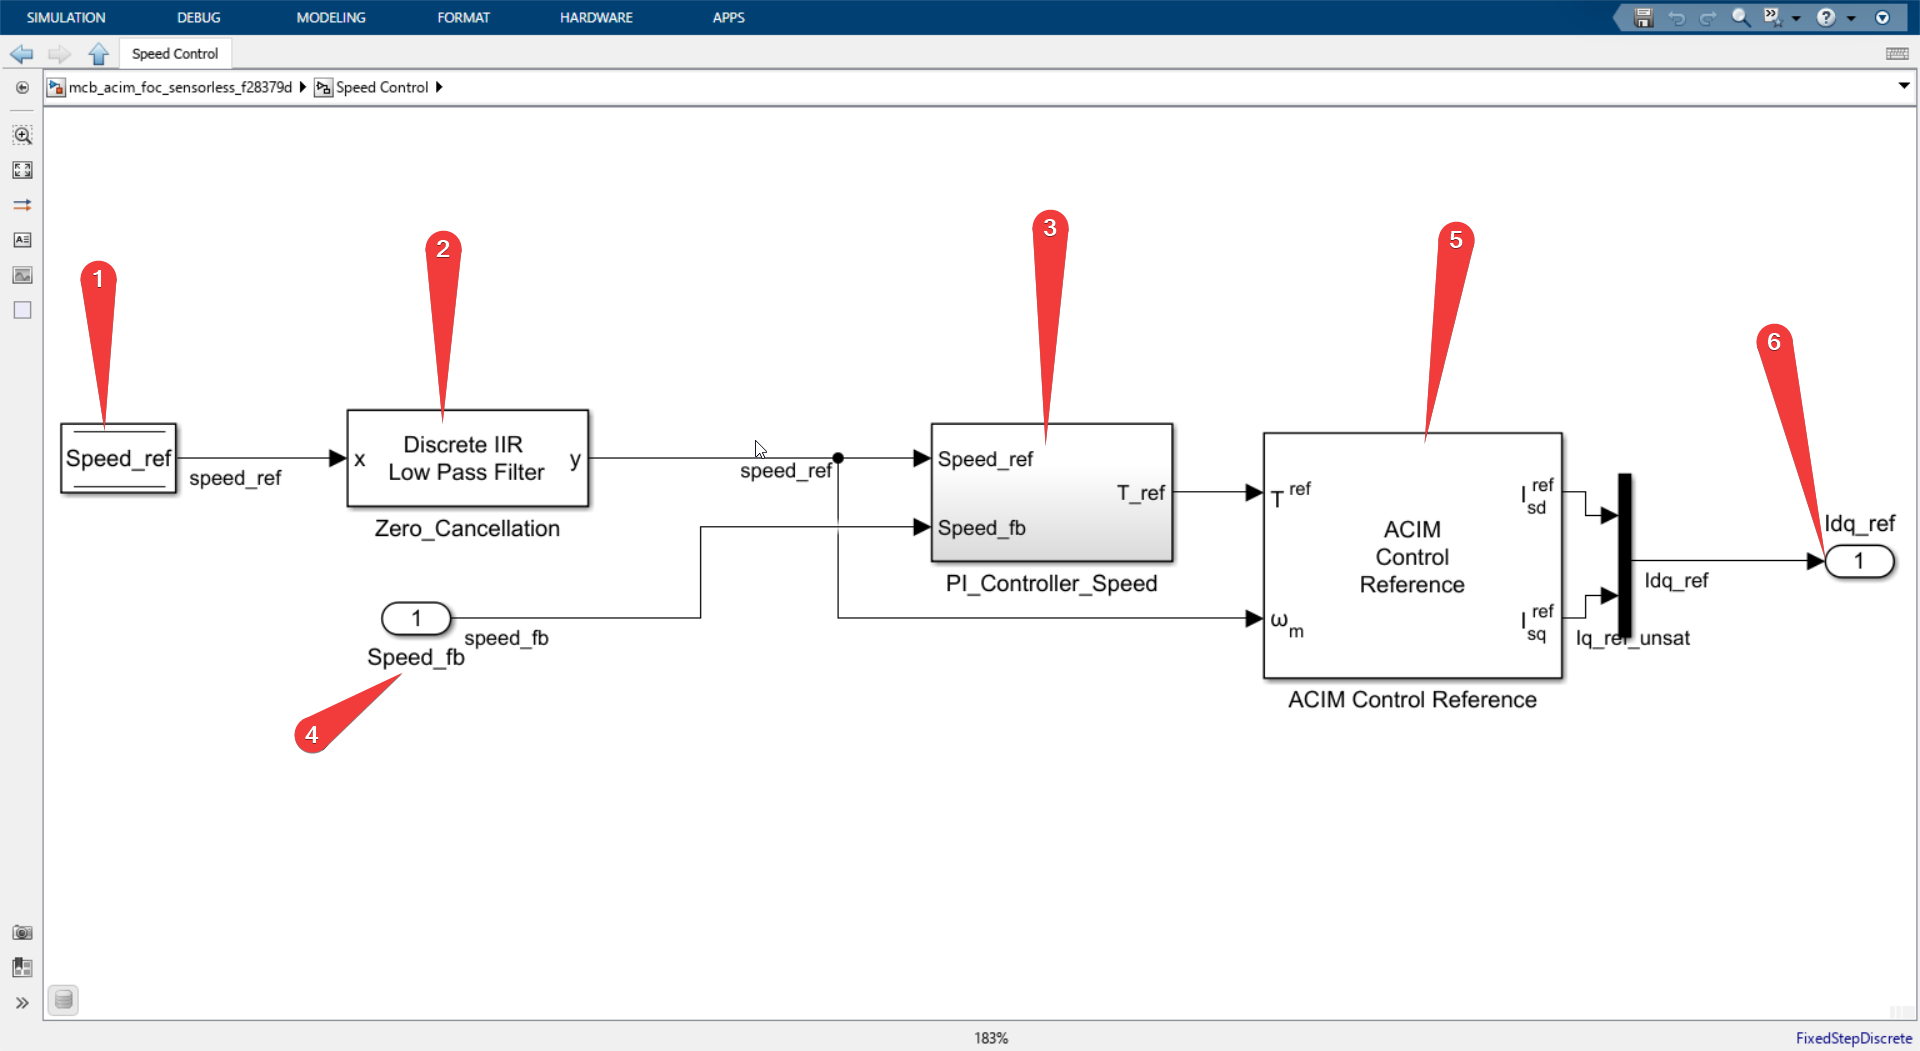
\includegraphics[width=4in]{sections/section3/images/simulation/speedControl/speedController.png}
	\caption{Speed Control System}
	\label{fig:speed_control_system}
\end{figure}


The speed control system shown in Figure \ref{fig:speed_control_system} consists of a DataStoreRead block that holds the speed reference value received from the host computer, a Discrete IIR lowpass filter block to cancel the zeros in the system, and a Discrete PID Controller with anti-windup block that takes the speed reference and feedback values as inputs and generates the torque reference as output. The ACIM Control reference block then takes the torque reference and speed reference as inputs and generates the $Isd_ref$ and $Isq_ref$ values, which are the reference values for the current control loop. The DQ limiter block is used to limit the magnitude of the vector represented in the d-q reference frame, with the option to prioritize either the d-axis or q-axis component.


\subsection{Current Control Subsystem}



\subsubsection{Control System}

\begin{figure}[H]
	\centering
	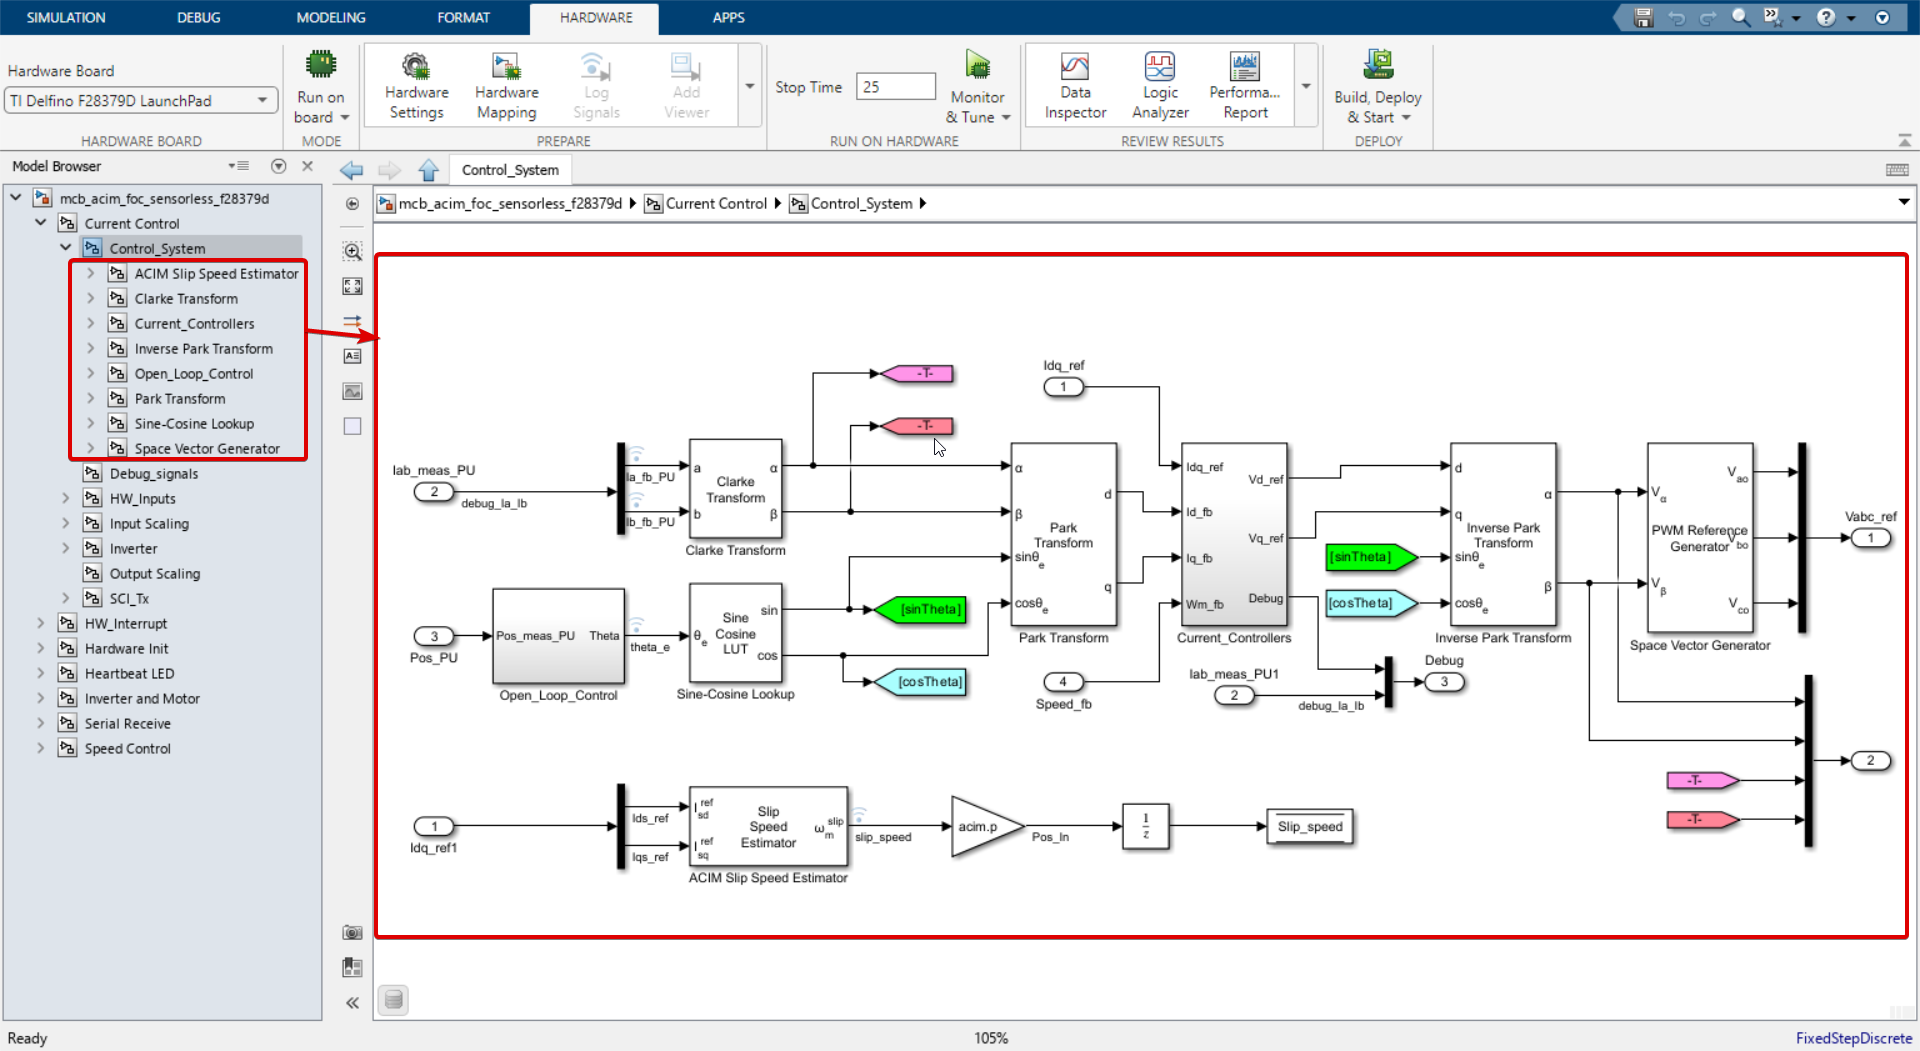
\includegraphics[width=4in]{sections/section3/images/simulation/currentControl/controlSystem.png}
	\caption{Current Control System}
	\label{fig:current_control_system}
\end{figure}


The control system shown in Figure \ref{fig:current_control_system} implemented in the inner current loop consists of two main components: the current controllers and the DQO transformation.

The current controllers use Proportional-Integral (PI) controllers to minimize the error between the reference currents ($I_{dq\_ref}$) and the feedback currents ($I_{d\_fb}$ and $I_{q\_fb}$). The output of the PI controllers is then limited, filtered, and adjusted using a feedforward controller and a saturation function to ensure safe and reliable operation of the system. The adjusted d-axis current is then used to generate the reference voltages ($V_{d\_ref}$ and $V_{q\_ref}$) in the DQ frame. These reference voltages are then transformed into the alpha-beta frame using the stator flux position ($\theta$) and fed into the PWM reference generator block, which generates the three-phase voltage references for the inverter. This inner current loop ensures that the actual currents closely follow the desired reference currents, which is crucial for the overall performance and stability of the control system.


\newpage